 % The main file for CAMP reports
 % Don't put any content in here. 
 % Don't even include content files by using \input or \inlcude. 
 % Put your content to TEXT.TEX or include it there using \input.
 % Uses:
 %		SETTINGS.TEX	contains the settings for this document
 %		COMMANDS.TEX	contains commands which can be used while writing
 %		INFO.TEX			contains the author, title and so on for the cover
 %		COVER.TEX			formats the front cover of the document
 %		ABSTRACT.TEX	contains the abstract to be included (if needed)
 %		TEXT.TEX			contains the actual content of the document
 %		BIB.BIB				containt the BibTeX entries for the document
 
 
%% Draft document mode
%% Final document
\documentclass[11pt,a4paper,bibtotoc,idxtotoc,headsepline,footsepline,footexclude,BCOR12mm,DIV13]{scrbook}

%\documentclass[11pt,a4paper,bibtotoc,idxtotoc,headsepline,footsepline,footexclude,BCOR20mm,DIV10]{scrbook}

% KOMA-Optionen:
%  bibtotoc: include bibliography in table of contents
%  idxtotoc: include index in table of contents
%  headsepline: use horizontalline under heading
%  BCOR: binding correcion (Bindungskorrektur) (e.g.: BCOR5mm)
%  DIV: Number of sheet sections (used for layout) (e.g.: DIV12) 



% include title and author information for the cover
% Set here the title, authors and other stuff to be used for the cover
% This file is used by MAIN.TEX

% set title, authors and stuff for the cover
\def\doctype{Bachelorarbeit in Informatik}
\def\title{Object detection and segmentation in cluttered scenes through perception and manipulation}
\def\titleGer{Objekterkennung und Segmentierung durch Perzeption und Manipulation}
\def\author{Julius Adorf}
\def\date{July 15, 2011}

% text to appear in the footer
\def\footertext{}


% include settings
% Included by MAIN.TEX
% Defines the settings for the CAMP report document

\renewcommand{\sectfont}{\normalfont \bfseries}        % Schriftart der Kopfzeile

% manipulate footer
\usepackage{scrpage2}
\pagestyle{scrheadings}
\ifoot[\footertext]{\footertext} % \footertext set in INFO.TEX
%\setkomafont{pagehead}{\normalfont\rmfamily}
\setkomafont{pagenumber}{\normalfont\rmfamily}

%% allow sophisticated control structures
\usepackage{ifthen}

% use Palatino as default font
\usepackage{palatino}

% enable special PostScript fonts
\usepackage{pifont}

% make thumbnails
\usepackage{thumbpdf}

%to use the subfigures
\usepackage{subfigure}


\usepackage{colortbl}


%% show program code\ldots
%\usepackage{verbatim}
%\usepackage{program}

%% enable TUM symbols on title page
\usepackage{styles/tumlogo}


\usepackage{multirow}

%% use colors
\usepackage{color}

%% make fancy math
\usepackage{amsmath}
\usepackage{amsfonts}
\usepackage{amssymb}
% mathtools necessary for dcases environment
% TODO: either remove mathtools.sty from styles or remove install statement in Makefile for texlive-latex3
\usepackage{styles/mathtools}
\usepackage{textcomp}
\usepackage{styles/yhmath} % f�r die adots 
%% mark text as preliminary
%\usepackage[draft,german,scrtime]{prelim2e}

%% create an index
\usepackage{makeidx}


% for the program environment
\usepackage{float}

%% load german babel package for german abstract
%\usepackage[german,american]{babel}
\usepackage[german,english]{babel}
\selectlanguage{english}

% use german characters as well
\usepackage[utf8]{inputenc}       % allow Latin1 characters

% use initals dropped caps - doesn't work with PDF
\usepackage{styles/dropping} % fix

\usepackage{styles/shortoverview}
%----------------------------------------------------
%      Graphics and Hyperlinks
%----------------------------------------------------

%% check for pdfTeX
\ifx\pdftexversion\undefined
 %% use PostScript graphics
 \usepackage[dvips]{graphicx}
 \DeclareGraphicsExtensions{.eps,.epsi}
 \graphicspath{{figures/}{figures/review}} 
 %% allow rotations
 \usepackage{rotating}
 %% mark pages as draft copies
 %\usepackage[english,all,light]{draftcopy}
 %% use hypertex version of hyperref
 \usepackage[hypertex,hyperindex=false,colorlinks=false]{hyperref}
\else %% reduce output size \pdfcompresslevel=9
 %% declare pdfinfo
 %\pdfinfo { 
 %  /Title (my title) 
 %  /Creator (pdfLaTeX) 
 %  /Author (my name) 
 %  /Subject (my subject	) 
 %  /Keywords (my keywords)
 %}
 %% use pdf or jpg graphics
 \usepackage[pdftex]{graphicx}
 \DeclareGraphicsExtensions{.jpg,.JPG,.png,.pdf,.eps}
 \graphicspath{{figures/}} 
 
 %% Load float package, for enabling floating extensions
 \usepackage{float}
 
 %% allow rotations
 \usepackage{rotating}
 %% use pdftex version of hyperref
 \usepackage[pdftex,colorlinks=true,linkcolor=red,citecolor=red,%
 anchorcolor=red,urlcolor=red,bookmarks=true,%
 bookmarksopen=true,bookmarksopenlevel=0,plainpages=false%
 bookmarksnumbered=true,hyperindex=false,pdfstartview=%
 ]{hyperref}
%
%\usepackage[pdftex,colorlinks=false,linkcolor=red,citecolor=red,%
% anchorcolor=red,urlcolor=red,bookmarks=true,%
% bookmarksopen=true,bookmarksopenlevel=0,plainpages=false%
% bookmarksnumbered=true,hyperindex=false,pdfstartview=%
% ]{hyperref}
\fi

%% Fancy chapters
%\usepackage[Lenny]{fncychap}
%\usepackage[Glenn]{fncychap}
%\usepackage[Bjarne]{fncychap}

%\usepackage[avantgarde]{quotchap}

% set the bibliography style
%\bibliographystyle{styles/bauermaNum}
%\bibliographystyle{alpha}
%\bibliographystyle{plain}
\bibliographystyle{ieeetr} % list citations in order of appearance

% Arnold Schwarzenegger trick: can be used to add some flexible space after
% command without the necessity of adding curly brackets when calling the
% command.
% see: http://stackoverflow.com/questions/512729/space-after-latex-commands
\usepackage{xspace}  



% include commands
% Commands to be used within the TUM report document
% Included by MAIN.TEX
% Please include your own cool commands here. 
% Be only sure to comment it sufficiently so others can use it.

%-------------------------------------------------------------
%                      Own Commands
%-------------------------------------------------------------

\newcommand{\clutseg}{{\tt CLUTSEG}\xspace} 	
\newcommand{\tod}{{\tt TOD}\xspace} 	
\newcommand{\oTvh}{_{o}\hat{T}^{v}}
\newcommand{\oTv}{_{o}T^{v}}
\newcommand{\vTo}{_{v}T^{o}} 	
\newcommand{\oTvi}[1]{_{o}T_{#1}^{v}} 	
\newcommand{\vToi}[1]{_{v}T_{#1}^{o}} 	
\newcommand{\fTv}{_{f}T^{v}}
\renewcommand{\vec}[1]{\mathbf{#1}}
\newcommand{\normtwo}[1]{{\left|\left| #1 \right|\right|}_{\mbox{\tiny 2}}} 	
\newcommand{\assamTea}{{\it assam\_tea}\xspace}
\newcommand{\haltbareMilch}{{\it haltbare\_milch}\xspace}
\newcommand{\jacobsCoffee}{{\it jacobs\_coffee}\xspace}
\newcommand{\icedtea}{{\it icedtea}\xspace}

%-------------------------------------------------------------
% math stuff -------------------------------------------------

% nice R, N, C
\newcommand{\nat}{\mathbb{N}}
\newcommand{\real}{\mathbb{R}}
\newcommand{\compl}{\mathbb{C}}



% norm
\newcommand{\norm}[1]{\left\| #1 \right\|}

% un demi
\newcommand{\half}{\frac{1}{2}}

% parantheses
\newcommand{\pth}[1]{ \left( #1 \right) }
\newcommand{\brt}[1]{ \left[ #1 \right] }
\newcommand{\cbr}[1]{ \left\{ #1 \right\} }
%\newcommand{\angle}[1]{ \left\langle  #1 \right\rangle }

% partial derivative: %#1 function, #2 which variable
% simple / single line version
\newcommand{\pardevS}[2]{ \delta_{#1} f(#2) }
% fraction version
\newcommand{\pardevF}[2]{ \frac{\partial #1}{\partial #2} }

% render vectors: 3 and 4 dimensional
\newcommand{\veciii}[3]{\left[ \begin{array}[h]{c} #1 \\ #2 \\ #3	\end{array} \right]}
\newcommand{\veciv}[4]{\left[ \begin{array}[h]{c} #1 \\ #2 \\ #3 \\ #4	\end{array} \right]}

% render matrices: 3  dimensional (arguments in row first order)
\newcommand{\matiii}[9]{\left[ \begin{array}[h]{ccc} #1 & #2 & #3 \\ #4 & #5 & #6 \\ #7 & #8 & #9	\end{array} \right]}
%DOESN'T WORK,DON'T KNOW WHY \newcommand{\mativ}[16]{\left[ \begin{array}[h]{cccc} #1 & #2 & #3 & #4 \\ #5 & #6 & #7 & #8 \\ #9 & #10 & #11 & #12 \\ #13 & #14 & #15 & #16 \end{array} \right]}


%-------------------------------------------------------------
%-------------------------------------------------------------


%-------------------------------------------------------------
% some abreviations ------------------------------------------
\newcommand{\Reg}{$^{\textregistered}$}
\newcommand{\reg}{$^{\textregistered}$ }
\newcommand{\Tm}{\texttrademark}
\newcommand{\tm}{\texttrademark~}
\newcommand {\bsl} {$\backslash$}

%-------------------------------------------------------------
%-------------------------------------------------------------


%-------------------------------------------------------------
% formating --------------------------------------------------

% Theorem & Co environments and counters
\newtheorem{theorem}{Theorem}[chapter]
\newtheorem{lemma}[theorem]{Lemma}
\newtheorem{corollary}[theorem]{Corollary}
\newtheorem{remark}[theorem]{Remark}
\newtheorem{definition}[theorem]{Definition}
\newtheorem{equat}[theorem]{Equation}
\newtheorem{example}[theorem]{Example}
\newtheorem{algorithm}[theorem]{Algorithm}

% inserting figures
\newcommand{\insertfigure}[4]{ % Filename, Caption, Label, Width percent of textwidth
	\begin{figure}[htbp]
		\begin{center}
			\includegraphics[width=#4\textwidth]{#1}
		\end{center}
		\vspace{-0.4cm}
		\caption{#2}
		\label{#3}
	\end{figure}
}




% referencing figures

\newcommand{\refFigure}[1]{ %label
	Figure~\ref{#1}
}
\newcommand{\refChapter}[1]{ %label
	Chapter~\ref{#1}
}

\newcommand{\refSection}[1]{ %label
	Section~\ref{#1}
}

\newcommand{\refParagraph}[1]{ %label
	Paragraph~\ref{#1}
}

\newcommand{\refEquation}[1]{ %label
	Equation~\ref{#1}
}

\newcommand{\refTable}[1]{ %label
	Table~\ref{#1}
}




\newcommand{\rigidTransform}[2]
{
	${}^{#2}\!\vec{H}_{#1}$
}

%code, in typewriter
\newcommand{\code}[1]
 {\texttt{#1}}

% comment that appears on the border - very practical !!!
\newcommand{\comment}[1]{\marginpar{\raggedright \noindent \footnotesize {\sl #1} }}

% page clearing
\newcommand{\clearemptydoublepage}{%
  \ifthenelse{\boolean{@twoside}}{\newpage{\pagestyle{empty}\cleardoublepage}}%
  {\clearpage}}


%-------------------------------------------------------------
%-------------------------------------------------------------


\newcommand{\etAl}{\emph{et al.}\mbox{ }}



%\makeindex
	%% inter line spacing
%\linespread{1.0}

\makeglossary

\begin{document}

	\frontmatter
	
	
	% The front cover for the TUM report document.
% Included by MAIN.TEX


%--------------------------------------------------
% The Front Cover
%--------------------------------------------------

% The front cover for the TUM document.
% Included by MAIN.TEX


%--------------------------------------------------
% The Front Cover
%--------------------------------------------------

% correct BCOR - undo at the end !!!
\def\bcorcor{0.15cm}
\addtolength{\hoffset}{\bcorcor}

\thispagestyle{empty}

 \vspace{4cm}
\begin{center}
	       \oTUM{4cm}
	   
	   \vspace{5mm}     
	   \huge FAKULT{\"A}T F{\"U}R INFORMATIK\\ 
	   \vspace{0.5cm}
	 \large DER TECHNISCHEN UNIVERSIT{\"A}T M{\"U}NCHEN\\
    \vspace{1mm}
        
	\end{center}
		

\vspace{15mm}
\begin{center}

   {\Large \doctype}

  \vspace{20mm}
  
  {\huge\bf \title}\\%[3ex]
  
  
  \vspace{15mm}
  
  
  {\LARGE  \author}
  
  \vspace{10mm}
  
  \begin{figure}[h!]
  \centering
   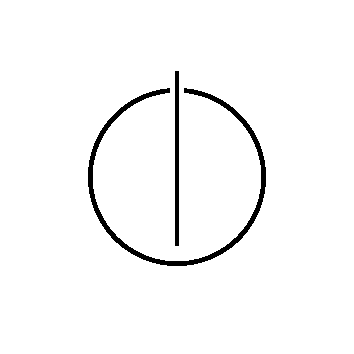
\includegraphics[width=4cm]{styles/informat.png}
  \end{figure}
  
  \end{center}
%	\clearemptydoublepage
%	
%	% The titlepage for the CAMP report document.
% Included by MAIN.TEX


%--------------------------------------------------
% The title page
%--------------------------------------------------

% correct BCOR - undo at the end !!!
\def\bcorcor{0.15cm}
\addtolength{\hoffset}{\bcorcor}

\thispagestyle{empty}

 \vspace{10mm}
\begin{center}
	       \oTUM{4cm}
	   
	   \vspace{5mm}     
	   \huge FAKULT{\"A}T F{\"U}R INFORMATIK\\ 
	   \vspace{0.5cm}
	 \large DER TECHNISCHEN UNIVERSIT{\"A}T M{\"U}NCHEN\\
        
	\end{center}
		

\vspace{10mm}
\begin{center}

   {\Large \doctype}

  \vspace{10mm}
  
  {\LARGE \title}\\
  
  
  \vspace{10mm}
  
  
  {\LARGE  \titleGer}\\
  
  
  \vspace{10mm}

    %\hfill
    \begin{tabular}{ll}
	   \Large Author:     & \Large \author \\[2mm]
	   \Large Supervisor:    & \Large Prof. Michael Beetz\\[2mm]				
	   \Large Advisor:	& \Large M.Sc. Dejan Pangercic\\[2mm]
	   \Large Date:       & \Large July 15, 2011
	 \end{tabular}
	 
	 \vspace{5mm}
	 
	 \begin{figure}[h!]
  \centering
   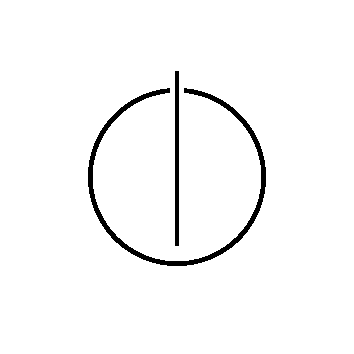
\includegraphics[width=4cm]{styles/informat.png}
  \end{figure}
   

\end{center}

% undo BCOR correction
\addtolength{\hoffset}{\bcorcor}

	
	
%	\input{components/cover_maschmeyer}
	\clearemptydoublepage
	
	% The titlepage for the CAMP report document.
% Included by MAIN.TEX


%--------------------------------------------------
% The title page
%--------------------------------------------------

% correct BCOR - undo at the end !!!
\def\bcorcor{0.15cm}
\addtolength{\hoffset}{\bcorcor}

\thispagestyle{empty}

 \vspace{10mm}
\begin{center}
	       \oTUM{4cm}
	   
	   \vspace{5mm}     
	   \huge FAKULT{\"A}T F{\"U}R INFORMATIK\\ 
	   \vspace{0.5cm}
	 \large DER TECHNISCHEN UNIVERSIT{\"A}T M{\"U}NCHEN\\
        
	\end{center}
		

\vspace{10mm}
\begin{center}

   {\Large \doctype}

  \vspace{10mm}
  
  {\LARGE \title}\\
  
  
  \vspace{10mm}
  
  
  {\LARGE  \titleGer}\\
  
  
  \vspace{10mm}

    %\hfill
    \begin{tabular}{ll}
	   \Large Author:     & \Large \author \\[2mm]
	   \Large Supervisor:    & \Large Prof. Michael Beetz\\[2mm]				
	   \Large Advisor:	& \Large M.Sc. Dejan Pangercic\\[2mm]
	   \Large Date:       & \Large July 15, 2011
	 \end{tabular}
	 
	 \vspace{5mm}
	 
	 \begin{figure}[h!]
  \centering
   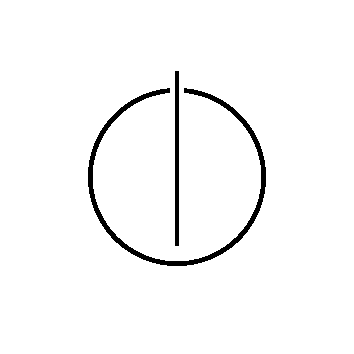
\includegraphics[width=4cm]{styles/informat.png}
  \end{figure}
   

\end{center}

% undo BCOR correction
\addtolength{\hoffset}{\bcorcor}

	
	
	\clearemptydoublepage


\thispagestyle{empty}
\selectlanguage{german}
	\vspace*{0.8\textheight}
	\noindent
	Ich versichere, dass ich diese Bachelorarbeit selbst{\"a}ndig verfasst und nur 
	die angegebenen \\Quellen und Hilfsmittel verwendet habe.
	
	\vspace{15mm}
	\noindent
	M{\"u}nchen, den 15. Juli \hspace{5cm} \author
\selectlanguage{english}
\newpage

	
	\clearemptydoublepage
\phantomsection
\addcontentsline{toc}{chapter}{Acknowledgements}	


%\chapter*{Acknowledgements}

\vspace*{2cm}

\begin{center}
{\Large \bf Acknowledgments}
\end{center}

\vspace{1cm}

\begin{center}
    To my family.
\vspace{1cm}
\end{center}

% M.K.
% L.C.G.
% D.P.
% H.M.A.
% G.A.
% C.S.
% T.R.
% A.S.
% E.R.
% V.R.
% M.C.B.

\vspace{1cm}


My family has patiently supported me during my four-month quest in science and
technology. My appreciation to my equally dear, and loyal friends, who I
certainly have met less often than I would have liked to.  Thanks to Dejan
Pangercic, my advisor, who was the first to introduce me into the challenges to
be found in the world of robotics and computer vision. Lucian Goron was never
short of pragmatic advice. Thumbs up for Manuel Baierl for finding a money- and
time-saving shortcut to the laboratory. The discussions with Martin Kreuzeder
helped to shape my understanding about geometry, proving useful in several
parts of this work.  Many thanks to Hans-Martin Adorf for his generous
comments, and his advice on style.  Thanks to Gabriel Adorf and Christian
Schöne, who both taught me about the importance of graphics, and the basics in
how to create them. Yet, my drawing are no match to theirs. Thanks to Chanrith
Siv for helping me to remove the roughest edges in my English writing. Thanks
to Alexander Shishkov, Ethan Rublee, and Vincent Rabaud for their comments on
software that was not supposed to be used by the public. Notably, the help of
Zoltan-Csaba Marton and Thomas Rühr, who helped me operating the robot at
Technische Universität München. Thank you.


	
	% Abstract for the TUM report document
% Included by MAIN.TEX


\clearemptydoublepage
% Enable when used with hyperref
% \phantomsection
\addcontentsline{toc}{chapter}{Abstract}	

\vspace*{2cm}
\begin{center}
{\Large \bf Abstract}
\end{center}
\vspace{1cm}

Recognition of textured objects is fundamental in many robotic applications in
household environments. This work addresses the perception task of finding a
rigid textured object and its 3D pose in a cluttered scene such that the
cluttered scene can subsequently be resolved by successive removal of objects
by a robot.

A system is presented that learns local 2D features and 3D models from objects.
It is able to detect an object and estimate its pose in a cluttered scene by
matching observed local 2D features against the learned models.  Confidence
values provide a measure of goodness for estimated object poses. For the object
with the highest confidence value, the pose is refined in order to reduce
error, and that estimate provides a basis for the grasping pipeline of a robot.
The system is based on the existing, yet immature and unstable textured object
recognition stack in the Robot Operating System. Recent developments in object
recognition are reviewed in this context, especially the Oriented BRIEF feature
detector and descriptor.

Experiments have shown that in 82\% of cluttered scenes in a validation set, an
object is correctly recognized in the scene within a margin for rotational
error of 20 degrees and for translational error of 3 cm.  A live test on the robot
revealed limitations as well as promising aspects of the approach.

\clearemptydoublepage
% Enable when used with hyperref
% \phantomsection
\addcontentsline{toc}{chapter}{Zusammenfassung}

\vspace*{2cm}
\begin{center}
{\Large \bf Zusammenfassung}
\end{center}
\vspace{1cm}


Die Erkennung von Objekten spielt in vielen Anwendungen der Robotik in
Haushalten eine wichtige Rolle. Diese Arbeit beschreibt die Aufgabe, die Lage
und Orientierung eines starren, texturierten Körpers in einer Szene mit vielen
weiteren Objekten zu bestimmen. Auf diese Art und Weise sollen die Objekte
nacheinander von einem Roboter entfernt werden können.

Ein System wird vorgestellt, welches lokale 2D-Merkmale und 3D-Modelle von
einem Objekt erstellt. Indem das System beobachtete lokale 2D-Merkmale mit den Modellen
assoziiert, kann es ein Objekt erkennen, und dessen Lage und Orientierung im
Raum bestimmen. Konfidenzwerte geben Aufschluss über die Zuverlässigkeit für
die Schätzungen der Lage und der Orientierung der Objekte.  Die erste Schätzung
mit dem höchsten Konfidenzwert wird verfeinert. Die verfeinerte Schätzung
reduziert den Fehler und ermöglicht dem Roboter, das Objekt zu greifen. Das
System beruht auf der bestehenden, noch nicht ausgereiften
Textured-Object-Recognition-Bibliothek aus dem Robot Operating System.  Jüngste
Entwicklungen aus der Objekterkennung werden vorgestellt, insbesondere darunter
der Oriented-BRIEF-Algorithmus zur Bestimmung und Beschreibung von lokalen
2D-Merkmalen.

Experimente zeigen, dass die Lage und die Orientierung eines Objekts in 82\%
der zur Validierung ausgewählten Szenen erfolgreich bestimmt werden, mit einer
Fehlertoleranz von 3 cm Versatz und 20 Grad Winkelunterschied. Ein Testlauf auf
dem Roboter zeigt sowohl Grenzen als auch vielversprechende Aspekte des
Ansatzes auf.



	\tableofcontents
  
  \clearemptydoublepage

\phantomsection
% \addcontentsline{toc}{chapter}{Outline}

\begin{center}
	\huge{Outline}
\end{center}

%--------------------------------------------------------------------
\section*{Part I: Introduction}

\noindent {\scshape Chapter 1: Statement of the Problem}  \vspace{1mm}

The reader learns about the outcome of the work, and about the contribution of
this work to the field. The reader learns about existing other work in this
area.

\noindent {\scshape Chapter 2: Intended Purpose}  \vspace{1mm}

The reader learns why this work has been done and where the system can be used.

\noindent {\scshape Chapter 3: Selected Approach}  \vspace{1mm}

The reader learns about the methods that have been employed.

%--------------------------------------------------------------------
\section*{Part II: Theory}

\noindent {\scshape Chapter 1: Object Recognition}  \vspace{1mm}

The reader learns about the terminology used in object recognition,
especially with regard to this paper. The reader learns about existing work in
object recognition that is important for this work. The reader learns about
different approaches to object recognition.

\noindent {\scshape Chapter 2: Classifier Evaluation}  \vspace{1mm}

The reader learns about the terminology used in classifier evaluation,
especially with regard to this paper. The reader learns about how to view
the object recognition task as a classification problem. 

%--------------------------------------------------------------------
\section*{Part III: Implementation}

\noindent {\scshape Chapter 1: Model Learning}  \vspace{1mm}

The reader learns about how models are generated that lay the foundation for
later classification. The reader learns how certain difficulties have been
resolved. The reader learns about the learning parameters and their effects.

\noindent {\scshape Chapter 2: Object Recognition}  \vspace{1mm}

The reader learns how the classification process works and how the pose of the
object is estimated. The reader learns about the design choices.  The reader
learns about the parameters that can be adjusted to get different classifiers.

\noindent {\scshape Chapter 3: Parameter Selection}  \vspace{1mm}

%--------------------------------------------------------------------
\section*{Part IV: Results}

\noindent {\scshape Chapter 1: Performance in Experiments}  \vspace{1mm}

The reader learns about performance on datasets. The reader learns about how much
influence 3d information in models has on classification. The reader learns about
how long classification takes. 

\noindent {\scshape Chapter 2: Future Work}  \vspace{1mm}

The reader learns which areas have not been sufficiently investigated into,
which issues remain and where to improve.

\noindent {\scshape Chapter 3: Conclusion}  \vspace{1mm}

The reader is reminded what this work was about. The reader learns about what is
different to other works and possible usage scenarios are presented.
% 
% %--------------------------------------------------------------------
% \section*{Part I: Introduction and Theory}
% 
% \noindent {\scshape Chapter 1: Introduction}  \vspace{1mm}
% 
% \noindent  This chapter presents an overview of the thesis and it purpose. Furthermore, it will discuss the sense of life in a very general approach.  \\
% 
% \noindent {\scshape Chapter 2: Theory}  \vspace{1mm}
% 
% \noindent  No thesis without theory.   \\
% 
% %--------------------------------------------------------------------
% \section*{Part II: The Real Work}
% 
% \noindent {\scshape Chapter 3: Overview}  \vspace{1mm}
% 
% \noindent  This chapter presents the requirements for the process.


	\mainmatter
	
	
		% ---------------------------------------------------------------------------
		%
		%Introduction and Background Theory
		%
		% ---------------------------------------------------------------------------
		\part[Introduction and Theory]{Introduction and Theory}
		\label{part:introAndBackgroundTheory}
		\chapter{Introduction}
\label{chapter:Introduction}



\section{What}
\section{Purpose}
\section{How}
 



		
		
		%
		%% ---------------------------------------------------------------------------
		%%
		%% Fully Automated Calibration for Ultrasound
		%%
		%%% ---------------------------------------------------------------------------
		\part[The 2nd Part]{The Second Part}
		\label{part:secondP}
		
		
		% ---------------------------------------------------------------------------
		%
		% Appendix
		%
		% ---------------------------------------------------------------------------
		
		\part*{Appendix}
		\addcontentsline{toc}{part}{Appendix}
		
		\appendix %---------------------------------------
		
		\chapter{Detailed Descriptions}
%\section{Detailed Validation Results}
\label{chapter:DetailedDescriptions}
Here come the details that are not supposed to be in the regular text.
		
	


  \clearemptydoublepage
  
	\bibliography{bibliography/literature}
	
 
\end{document}

